% !TeX program = xelatex
% !BIB program = biber
\documentclass[a4paper, 12pt]{article}

\usepackage[brazil]{babel}
\let\latinencoding\relax
\usepackage[T1]{fontenc}

% Fontes.
\usepackage{fontspec}
\usepackage{lmodern}
%\usepackage{newpxtext, newpxmath}

% Define as margens.
\usepackage[a4paper, margin=2cm]{geometry}
\usepackage{csquotes}
\usepackage{pdflscape}
\usepackage{graphicx}
\usepackage{float}
\usepackage{booktabs}

% Importa o arquivo de definições, com dados dos autores.
\input{definition.tex}

\title{\titulo}
\author{\nomeAutorUm \and \nomeAutorDois}
\date{\today}

% Define as configurações do hyperref.
\usepackage{hyperref}
\hypersetup{
  colorlinks,
  urlcolor=blue,
  linkcolor=black,
  citecolor=black
}

% Define as configurações do minted.
\usepackage{minted}
\setminted{
  autogobble,
  frame=lines,
  framesep=2mm,
  baselinestretch=1.2,
  fontsize=\footnotesize,
  linenos,
  style=vs
}
% Redefine a exibição da contagem de linhas.
\renewcommand{\theFancyVerbLine}{\ttfamily{\scriptsize\arabic{FancyVerbLine}}}

% Bibliografia estilo ABNT.
\usepackage[style=abnt, language=brazil, scbib, giveninits, uniquename=init]{biblatex}
\addbibresource{bibliography.bib}

% Título personalizado.
\newcommand{\printtitle}{
  \begin{center}
    {\Large \scshape \titulo}\\[1em]
    {\nomeAutorUm, \raAutorUm}\\
    {\nomeAutorDois, \raAutorDois}\\
    {\nomeAutorTres, \raAutorTres}\\[1em]
    Professor: Dr\@. \nomeProfessor, \centroProfessor\\ 
    {\itshape \campusFaculdade}
  \end{center}
}

\begin{document}
  \printtitle

  \section{Descrição}

  O \emph{JavaScript Object Notation}, popularmente conhecido
  como JSON, é um padrão de troca rápida de informações
  criado no início dos anos 2000 por Douglas Crockford.
  O formato consiste de pares de atributo-valor, sendo
  comumente utilizado em aplicações \emph{web} através
  de requisições assíncronas entre cliente e servidor
  para consumo de APIs.
  
  \begin{minted}[label={Exemplo de um arquivo JSON}]{json}
    {
      "nome": "Universidade Federal do ABC",
      "sigla": "UFABC",
      "endereco": {
        "logradouro": "Avenida dos Estados",
        "numero": 501,
        "municipio": "Santo André",
        "estado": "São Paulo"
      }
    }
  \end{minted}
  
  A utilização do JSON em um banco de dados ocorre
  principalmente pela sua performance nas consultas e 
  pela sua fácil manutenção, agilizando o processo de
  desenvolvimento e futuras mudanças no banco \cite{smith16}.
  Em alguns bancos de dados é possível notar que existem 
  dados que dependem um do outro, onde, na grande maioria 
  das vezes, são sempre consultados juntos, mas que pelas 
  regras de normalização, não estão na mesma relação, o 
  que infere na utilização de um \verb|join| nessa consulta, 
  tornando essa consulta mais custosa e ineficaz. Tal problema
  pode ser facilmente contornado com o armazenamento 
  do JSON em uma coluna da relação com os dados que 
  ``pertencem a ela''.
  
  Outro fator que torna o JSON uma opção muito viável é
  a agilidade do desenvolvimento que esse proporciona.
  Mudanças pontuais podem ser feitas sem a alteração do 
  \emph{squema}, uma operação trabalhosa dependendo
  da quantidade de relações que um banco possui e da
  quantidade de aplicativos e \emph{softwares} que 
  compartilham esse banco, pois a alteração de algum
  atributo/parâmetro pode ser feita apenas a partir 
  da alteração do JSON sem que a necessidade da 
  alteração do \emph{squema} relacional.
  
  O PostgreSQL a partir da versão 9.2 \cite{halliday2018}
  possui dois tipos de dados especializados em 
  armazenar o padrão JSON: o \verb|json| e \verb|jsonb|.
  A principal diferença entre ambos é o custo. 
  Como o \verb|json| é armazenado como ele é, ou seja, 
  em formato de texto, sua inserção e alteração são 
  rápidas, mas a consulta precisa toda vez processar
  o texto armazenado. O \verb|jsonb| busca eliminar
  este custo adicional nas consultas e, durante
  a inserção e alteração, faz um único processamento
  convertendo o dado para binário, o que permite
  uma melhora muito significativa nas consultas
  \cite{pddatatypejson}.
  
  Dado um registro já armazenado do tipo \verb|json|
  ou \verb|jsonb|, é possível manipulá-lo em consultas
  diretamente, sem ter a necessidade de usar alguma
  biblioteca externa, utilizando operadores no PostgreSQL.
  Isto será demonstrado na seção Caso-Exemplo.

  \section{Caso-Exemplo}
  
  Para demonstrar a utilização do tipo \verb|jsonb|,
  foi criado um banco de dados com três tabelas,
  com uma pequena relação entre si, que simulam
  um sistema bem simples de pedidos.
  
  \begin{figure}[h!]
    \centering
    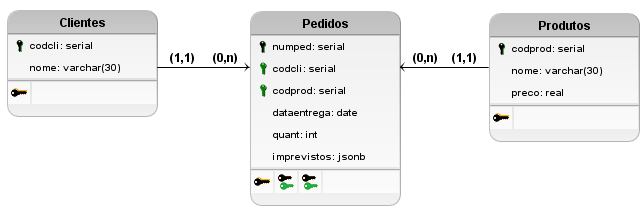
\includegraphics[width=0.8\linewidth]{example-case.png}
    \caption{Modelo lógico do banco de dados.}
    \label{fig:my_label}
  \end{figure}
  
  Essas tabelas foram populadas com dados de exemplo,
  sendo \verb|Pedidos| a tabela mais importante, 
  que contém a coluna \verb|imprevistos|,
  do tipo \verb|jsonb|. Esta coluna foi preenchida
  com JSON's variados, como os da Tabela \ref{tab:ex}.
  
  \begin{table}[h!]
    \centering
    \begin{tabular}{ccl}
      \toprule
      \texttt{numped} & $\cdots$ & \texttt{imprevistos} \\
      \midrule
      1 & $\cdots$ & \mintinline{json}{{"adicionais": ["ar condicionado", "airbag"]}} \\
      2 & $\cdots$ & \mintinline{json}{{"entrega": "atrasada"}} \\
      3 & $\cdots$ & \mintinline{json}{{"pedido": "expirado"}} \\
      4 & $\cdots$ & \mintinline{json}{{"caminhao": "danificado", "motorista": "multado"}} \\
      $\vdots$ & $\cdots$ & \hspace{0.2cm} $\vdots$ \\
      \bottomrule
    \end{tabular}
    \caption{Exemplos populados na tabela \texttt{Pedidos}.}
    \label{tab:ex}
  \end{table}
  
  É possível, então, realizar consultas utilizando os
  operadores de \verb|jsonb| que o PostgreSQL oferece.
  Por exemplo, pode-se buscar os clientes que tiveram
  problemas relacionados aos caminhões da entrega
  do pedido:
  
  \begin{figure}[h!]
    \centering
    \begin{minted}{postgres}
      select cli.nome cliente, prod.nome produto, ped.imprevistos->>'caminhao' caminhao
      from clientes cli inner join pedido ped on cli.codcli = ped.codcli
      inner join produto prod on prod.codprod = ped.codprod
      where ped.imprevistos ? 'caminhao';
    \end{minted}
    \begin{tabular}{lll}
    \toprule
    \texttt{cliente} ($varchar(30)$) & \texttt{produto} ($varchar(30)$) & \texttt{caminhao} (\textit{text}) \\
    \midrule
    Robson Pereira & Bloco de folhas & danificado \\
    Nelson Santos & Mochila & roubado \\
    Judson Silva & Mochila & roubado \\
    \bottomrule
    \end{tabular}
  \end{figure}
  
  Neste exemplo, o operador \verb|->>| é utilizado.
  Este operador acessa o \verb|jsonb| armazenado em busca
  da chave passada logo em seguida, retornando seu valor
  em formato de texto caso exista, ou \verb|null| caso
  não exista \cite{pdfunctionjson}. Como queremos apenas 
  os registros de \verb|Pedidos| que tenham a chave
  \verb|caminhao| em \verb|imprevistos|, precisamos 
  filtrar apenas estas. Isto é feito utilizando o
  operador \verb|?|, que verifica se uma chave dada
  existe em um campo do tipo \verb|jsonb|.
  
  Um caso usual seria a necessidade de ter que adicionar
  um novo par chave-valor a um campo já preenchido.
  Por exemplo, pedidos podem sofrer atrasos de entrega
  devido a uma greve, então deve-se adicionar uma chave
  \verb|atraso| que informará quantos dias a mais
  o pedido demorará para ser entregue.
  
  \begin{minted}{postgres}
    update pedidos set imprevistos = imprevistos || '{"atraso": 5}';
  \end{minted}
  
  Neste caso, todos os pedidos sofreriam de um atraso
  de 5 dias, então não é especificado uma condição
  no \verb|update|. Usa-se o operador \texttt{||} para
  concatenar um \verb|jsonb| com um outro valor JSON,
  seja este em formato de texto, como o do exemplo, ou
  diretamente um \verb|jsonb|, como de outro campo, por
  exemplo \cite{huchet17}. Após a execução, todos os
  registros que não eram nulos, terão em seu campo
  \verb|imprevistos| uma nova chave \verb|atraso| 
  com o valor \verb|5|.
  
  Além dos operadores, o PostgreSQL oferece funções
  \emph{built-in} que também podem manipular os tipos 
  JSON \cite{pdfunctionjson}. Algumas vezes, um JSON
  pode conter uma chave cujo valor seja um vetor, 
  seja de objetos ou de tipos primitivos. Por exemplo,
  o pedido 1 possui  \verb|adicionais|, que é um vetor 
  de textos.  Pode-se então obter estes adicionais.
  
  \begin{figure}[h!]
    \centering
    \begin{minted}{postgres}
      select jsonb_array_elements_text(imprevistos->'adicionais') adicionais 
      from pedido where numped = 1;
    \end{minted}
    \begin{tabular}{l}
      \toprule
      \texttt{adicionais} (\textit{text}) \\
      \midrule
      ar condicionado \\
      airbag \\
      \bottomrule
    \end{tabular}
  \end{figure}
  
  Esta \emph{query} necessita a utilização do operador
  \verb|->|, que retorna o valor da chave passada como
  um objeto JSON, e não como texto, permitindo com
  que possa-se fazer manipulações em sub-objetos.
  A função \verb|jsonb_array_elements_text| interpreta
  o objeto passado, que deve ser um vetor, e retorna
  uma lista com o conteúdo do mesmo em texto. 
  Analogamente, existe a função \verb|jsonb_array_elements|
  que retorna uma lista de objetos JSON do vetor.
  
  \section{Conclusão}
  
  O JSON se tornou uma maneira simplificada de comunicação
  e armazenamento de informações. Utilizá-lo em um
  banco de dados como o PostgreSQL pode trazer benefícios
  principalmente em casos de incerteza de modelagem
  por parte do \emph{designer} do banco de dados.
  Isto não dificulta a consulta aos dados armazenados,
  já que os operadores e funções oferecidas ajudam em sua
  manipulação, evitando o uso de bibliotecas externas
  e melhorando a performance.

  % Imprime as referências bibliográficas.
  \printbibliography
\end{document}
